% *******************************************************************************
% * Copyright (c) 2007 by Elexis
% * All rights reserved. This document and the accompanying materials
% * are made available under the terms of the Eclipse Public License v1.0
% * which accompanies this distribution, and is available at
% * http://www.eclipse.org/legal/epl-v10.html
% *
% * Contributors:
% *    G. Weirich
% *
% *  $Id: multiuser.tex 2572 2007-06-23 11:09:43Z rgw_ch $
% *******************************************************************************
% !Mode:: "TeX:UTF-8" (encoding info for WinEdt)

\section{Einführung}
\index{Gemeinschaftspraxis}\index{Gruppenpraxis}\index{Gesundheitszentrum}
Elexis ist von Haus aus auf Mehrbenutzer- und Mehrmandantenbetrieb ausgelegt.
Es gibt dabei keine Beschränkung der Zahl der Anwender oder Mandanten. Es sind
auch keine besonderen Vorkehrungen notwendig, um vom Einzel- auf den
Mehrbenutzerbetrieb umzustellen. In diesem Kapitel müssen deshalb lediglich
einige Konzepte vorgestellt werden, welche im Mehrbenutzer- und
Mehrmandantenbetrieb nützlich sein können.

\section{Gruppen und Rechte}
\label{sec:gruppen}
Sobald mehr als ein Anwender auf den gemeinsamen Datenbestand zugreift, stellt
sich die Frage, welche Daten jeder Anwender lesen, schreiben oder löschen können
soll. Im Allgemeinen gilt das Prinzip, dass jeder das kann, was er
zur Erledigung seiner Arbeit braucht, aber möglichst nicht mehr. Dies reduziert
die Möglichkeit von Fehlbedienungen und erleichtert im Problemfall die Suche
nach den Ursachen.

Bei Elexis kann jeder Anwender Mitglied einer oder mehrerer Gruppen sein. Eine
Gruppe ist ein frei wählbarer Bezeichner, der keine weitere Funktion hat als
die, Anwender mit gemeinsamen Rechten zusammenzufassen. In einer grösseren
Arztpraxis könnte es beispielsweise die Gruppen 'MPA', 'Labor', 'Arzt' und
'Buchhaltung' geben, in einer Einzelpraxis vielleicht nur die Gruppen 'MPA' und
'Arzt'. Elexis bringt als Standardausstattung die Gruppen 'Anwender' und 'Admin'
mit.

Sobald Anwender und Gruppen definiert sind, können die Rechte verteilt werden.
Dieser Schritt ist unter Standardbedingungen nicht unbedingt notwendig, da die
normalerweise existierenden Rechte oft schon für diese Zwecke richtig definiert
sind.

Die Verteilung von Zugriffsrechten erfolgt über das Menü \textsc{Datei -
Einstellungen - Gruppen und Rechte - Zugriffsteuerung} (S. \ref{fig:zugriff}).
%\usepackage{graphics} is needed for \includegraphics
\begin{figure}[htp]
\begin{center}
  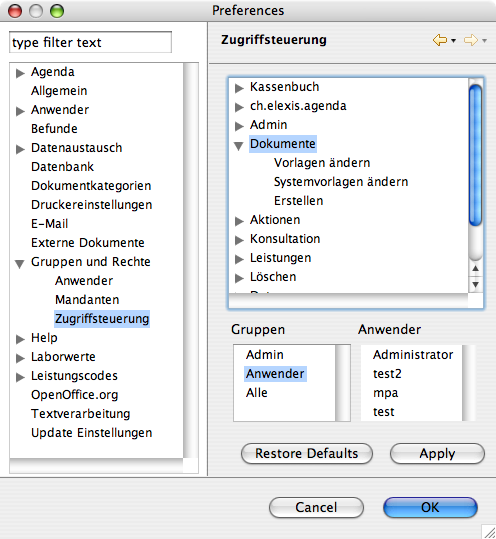
\includegraphics{images/zugriff}
  \caption{Zugriffssteuerung}
  \label{fig:zugriff}
\end{center}
\end{figure}

Wie Sie erkennen können, sind die Rechte benannt und hierarchisch angeordnet -
Das Recht \glqq Vorlagen ändern\grqq{} ist offensichtlich dem Recht \glqq
Dokumente\grqq{} untergeordnet. Im unteren Abschnitt des Fensters sehen Sie alle
im System vorhandenen Gruppen und Anwender. 
Die Regel ist nun so:
\begin{itemize}
  \item Wer ein Recht hat, hat implizit auch alle diesem Recht untergeordneten
  Rechte.
  \item Wer ein Recht hat, hat aber \textit{nicht} automatisch die diesem Recht
  übergeordneten Rechte.
  \item Jeder hat die Rechte aller Gruppen, denen er angehört, und zusätzlich
  diejenigen Rechte, die ihm individuell zugesprochen wurden.
  \item Wer zur Gruppe \glqq Admin\grqq gehört, hat sämtliche Rechte, auch wenn
  sie ihm nicht explizit erteilt wurden.
  \item Wer das Recht \glqq Zugriff - Rechte erteilen\grqq hat, kann sebst
  Zugriffsrechte verwalten, auch wenn er kein Administrator ist.
\end{itemize}

Man kann Zugriffrechte also an Gruppen oder an einzelne Anwender erteilen. Jedes
Recht kann an keine oder beliebig viele Gruppen und/oder Anwender erteilt
werden. Dies geschieht, indem man zunächst das Recht im oberen Feld anklickt,
und dann im untern Feld m it der linken Maustaste oder [STRG]+linke Maustaste
eine oder mehrere Gruppen oder Anwender auswählt.

\textbf{Wichtig:}Beherzigen Sie bitte folgende Grundregel: Niemand, auch der
Chef nicht, sollte für die tägliche Arbeit als Admin oder Mitglied der Gruppe
Admin angemeldet sein. Die Gefahr, mal schnell einen Fehler zu machen, der
wichtige Daten löscht, ist zu gross. Erstellen Sie als Praxisoberhaupt für sich
selbst zwei verschiedene Benutzerkonten (accounts):
\begin{itemize}
  \item Einen normalen Benutzer (z.B. Dr. Test), der der Gruppe Anwender oder
  Ärzte, aber jedenfalls nicth Admin angehört, und der genau diejenigen Rechte
  hat, die er für die Alltagsarbeti braucht.
  \item Einen Administratorbenutzer (z.B. Praxisadmin), der der Gruppe Admin
  angehört, und dessen Passwort Sie strikt für sich behalten, auch wenn Sie
  allen Mitarbeitern und Mitarbeiterinnen voll vertrauen. Logen Sie sich mit
  diesem account nur dann ein, wenn Sie wirklich mal Dinge tun müssen, die mit
  dem normalen Account nicht möglich sind.
\end{itemize}

\section{Definierbare Anwendereinstellungen}
In einer kleinen Praxis wird oft die Möglichkeit von Elexis geschätzt, den
Arbeitsplatz ganz individuell einzurichten. Die MPA kann ihren Bildschirm mit
anderen Farben und anderen Layouts gestalten, als die Ärztin.
In einem grösseren Betrieb, in dem vielleicht auch die Anwender zwischen
verschiedenen Arbeitsplätzen wechseln müssen, ist dagegen oft eine einheitliche
Gestaltung für alle, oder zumindest eine einheitliche Gestaltung je
Funktionsgruppe erwünscht. Elexis kommt diesem Wunsch mit konfigurierbaren
Farben und Layouts entgegen.

\subsection{Individuelle Programmeinstellungen}
In den Unterseiten von \textsc{Datei - Einstellungen - Anwender} können Sie
Farbdesigns, Tastenkürzel und Art der Schnellstartleiste definieren. Sie können
diese Einstellungen unter einem frei definierbaren Namen speichern. Geben Sie
dazu einen Namen ein und klicken Sie auf \glqq Einstellungen speichern
nach\grqq{}. 

Von einer anderen Arbeitsstation oder einem anderen Benutzeraccount aus können
Sie dieselben Einstellungen unter diesem Lamen wieder laden. Geben Sie dazu den
Namen ein und klicken Sie auf \glqq Einstellungen laden von\ldots\grqq{}.

\subsection{Definierbare Perspektivenlayouts}
Die Fensteranordnung, also die Perspektive, mit der Sie normalerweise arbeiten,
lässt sich ja auch individuell einstellen. Diese EInstellung ist an den
Arbeitsplatz gebunden (da sie ja auch von der Art des angeschlossenen Monitors
abhängt). Sie können aber auch die Perspektivenanordung unter einem Namen
speichern, um sie auf einen anderen Arbeitsplatz zu replizieren. Geben Sie
einfach den gewünschten Namen ein  und klicken Sie auf \glqq
Arbeitsplatzeinstellungen speichern nach\ldots\grqq{}.

Um die Perspektive auf einen anderen Arbeitsplatz zu kopieren, geben Sie dort
unter \textsc{Datei - Einstellungen - Anwender} den vorher vergebenen Namen ein
und klicken auf \glqq Arbeitsplatzeinstellungen laden von\grqq{}.


